% AIML ICGST LaTeX Template 
\section{Theory}
\label{Sec:Th}
There are two different approaches to the characterization of dynamic systems: In linear systems theory, one can assume either some structure in the signals or some structure in the system. Attempts have been made to combine these two approaches e.g. harmonic identification techniques in the Fourier domain.\\ 
\textbf{\textit{First approach:}} Structure the signal can be found using linear transforms. This approach does not take into account that the system has some structure. In the time domain, filtering is a linear transformation. The Fourier, Wavelet, and Karhunen-Loeve transforms have compression Capability and can be used to identify some structure in the signals. When we are using these transforms, we do not take into account any structure in the system.\\ 
\textbf{\textit{Second approach:}} Structure the system can be found by fitting a model to the system. 

\subsection{System Modeling}
Physical models of robots are either reduced-size copies of the original dynamics following the laws of model similarity, or analogies. The idea of an analogy implies that there exists "something" at every instant of time that is to be analogous to the dependent variables of the original physical system. Mathematical models map the relationships between the physical variables in the robot dynamics to be modeled onto mathematical structures like simple algebraic equations, systems of differential equations or even  difference equations. Mathematical modeling of robots can be developed in different ways: either purely theoretically based on the physical relationships (sensors actuators Interaction), which are a priori known about the robot dynamics, or purely empirically by experiments on the already existing robot, or by a sensible combination of both ways. Models obtained by the first method are often called priori, first principle or theoretical models, while models obtained in the second way are called posteriori or experimental models. Theoretical model building becomes unavoidable if experiments in the respective system cannot or must not be carried out. If the system to be modeled does not yet exist, theoretical modeling is the only possibility to obtain a mathematical model.

\subsection{ARX Modeling}
The discrete ARX modeling scheme  is derived from Kalman filter, see figure (\ref{fig:ARX}). The ARX scheme is widely used in modeling of sequential  system dynamics. This structure takes into account both the observed state $\upsilon_{k}$ and
the driving control signal $\lambda_{k}$ which is given by:
\begin{equation}
\upsilon_k = \sum\limits_{i = 1}^{n_a } {a_i \upsilon_{(k - i)} + } \sum\limits_{i =
0}^{n_b } {b_i \lambda_{(k - i)} + } \eta_k
\label{eq:ARX1}
\end{equation}

\begin{figure}[ht!]
\centering
\scalebox{1.00}{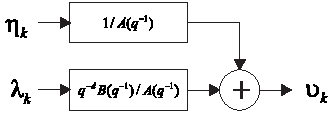
\includegraphics{pics/ARX}}
\caption{ARX modeling of rescue robot dynamics}
\label{fig:ARX}
\end{figure}

Where; $\eta$ is  the modeling residual , representing the white noise. $n_a$ is the model order of the observed state (also called the number of poles). $n_b$ is the model order of the control signal (also called the number of zeros). The operator $q^{-1}$  is the back shift operator or delay, which is given by $q^{ - 1}\upsilon_k = \upsilon_{(k - 1)} $,  that follows: 

\begin{equation}
\begin{array}{l}
A(q^{ - 1})\upsilon_k = q^{ - 1}B(q^{ - 1})\lambda_k + \eta_k \\
A(q^{ - 1}) = 1 - a_1 q^{ - 1} - a_2 q^{ - 2} - \ldots - a_{n_a } q^{ - n_a
} \\
B(q^{ - 1}) = b_0 + b_1 q^{ - 1} + b_2 q^{ - 2} + \ldots + b_{n_a } q^{ -
n_b } 
 \end{array}
 \label{eq:ARX2}
\end{equation}

The observed state $\upsilon_{k}$ is the longitudinal velocity/heading while the reference signal $\lambda_{k}$ is the obstacles distribution histogram, acquired by laser/sonar. The Gaussian distributed noise, associated with the observed output, facilitates applying identification algorithms such as; RLS or least mean squares (LMS) to estimate model parameters (coefficients).  This modeling scheme is only applicable within linear or quasi-linear systems. Therefore, it is applied  within this framework to regulate the velocity/heading, while this algorithm failed to cope with position control due to enormous non-linear odometric errors \cite{Buauthor_98, Jauthor_001, Sauthor_011, Rauthor_901, Sauthor_021, Abauthor_2003_13, Boauthor_971, kauthor_2002}. \\

Important Topics:
\begin{itemize}
	\item Item 1.
	\item Subject 2.
	\item New Data.
\end{itemize}
